\documentclass{article}

\usepackage{amsmath}
\usepackage{mdframed}

\newcommand{\irow}[1]{% inline row vector
  \begin{smallmatrix}[#1]\end{smallmatrix}%
}

\usepackage{xfrac}
\usepackage{bbm}
\usepackage{multicol}
\usepackage{geometry}
\usepackage{multirow}
\usepackage{lscape}
\geometry{margin=1in}



\providecommand{\e}[1]{\ensuremath{\times 10^{#1}}}

\title{F100-PW-220 Nozzle Optimization Problems}
\author{Richard W. Fenrich\\Department of Aeronautics and Astronautics\\Stanford University, Stanford, CA\\rfenrich@stanford.edu}
\date{May 24, 2016}

\begin{document}

\maketitle

\section{Overview}
This document provides background on the formulation of optimization problems for the design of a F100-PW-220 nozzle with uncertain parameters and provides several example optimization problems. The general form of the nozzle design optimization problem we are considering is:

\begin{equation}
\label{eq:generalFormulation}
%\mathbbm{P}_1 \begin{cases}
\begin{aligned}
& \underset{x}{\text{minimize}}
% objective function:
& & W(x)  \\
& \text{subject to}
% constraints:
& &  P [ T(x,\xi) \geq T_{req} ] > c_1 \\
& & & P [ N_f(x,\xi) \geq N_{f,min} ] > c_2 \\
& & & P [ max( T_w (x,\xi) ) \leq T_{max} ] > c_3 \\
& & & P [ max( \sigma_1 (x,\xi) ) \leq \sigma_{y} ] > c_4 \\
& & & A x \leq b \\
& & & l \leq x \leq u \\
\end{aligned}
%\end{cases}
\end{equation}

where $x$ denotes the vector of design variables (deterministic or otherwise) and $\xi$ denotes the random parameters.

The objective is weight $W(x)$ (or correspondingly volume of material), which does not depend on any random parameters.

There are four nonlinear stochastic constraints formulated as chance constraints:
\begin{enumerate}
\item Maintain adequate thrust $T(x,\xi)$ greater than the required thrust $T_{req}$. $T_{req}$ is determined by the aircraft's mission.
\item Ensure the nozzle's minimum number of cycles to failure $N_f(x,\xi)$ is greater than the minimum required number $N_{f,min}$. $N_{f,min}$ is a constant applicable to all missions.
\item Ensure the wall temperature $T_w(x,\xi)$ does not exceed the maximum allowable wall temperature $T_{max}$. $T_{max}$ is a material property.
\item Ensure the largest principle stress $\sigma_1(x,\xi)$ does not exceed the constant yield stress $\sigma_y$ of the material. $\sigma_y$ is also a material property, although this could change with temperature.
\end{enumerate}

The right hand side of the constraints $c = \irow{c_1 & c_2 & c_3 & c_4 }^T$ can be chosen for example, so that all $c_i = 0.99$.

In addition there are numerous linear constraints formulated as $A x \leq b$ which ensure the values of design variables lead to reasonable shapes. Section \ref{sec:linearConstraints} describes these in more detail.

Finally the design variables are bounded.

Implicit to the above optimization formulation are the distributions of the random parameters $\xi$ as well as any deterministic parameters required as inputs to the evaluation of any function.

\section{Variables}

The variables present in this nozzle design problem include those related to geometry, supporting structure, material, inlet conditions, and the environment.

\begin{mdframed}
\textbf{A note on definitions:} \textit{Design variables} are considered to be able to be actively changed by the optimization algorithm during the course of an optimization to improve the objective function. On the other hand, \textit{parameters} are considered to be unable to be changed during an optimization, although they influence the outcome. Both \textit{design variables} and \textit{parameters} can be considered \textit{variables} in the sense that they can vary. Both \textit{design variables} and \textit{parameters} can be deterministic or stochastic. In addition, some variables can be either a \textit{design variable} or a \textit{parameter}, such as the inlet radius of the nozzle.
\end{mdframed}

\subsection{Descriptions}

\subsubsection{Nozzle shape}
The shape of the nozzle's interior wall is parameterized using a 3rd-order basis spline (B-spline). In addition, the shape of the nozzle's wall thickness is parameterized using a piecewise-linear function. The nozzle is assumed to be radially symmetric.
\begin{description}
\item[Interior wall B-spline control points $c$] These control points are the set of coordinates contained in the coefficients matrix of the B-spline definition. They govern the shape of the interior wall of the nozzle and therefore govern important parameters such as: nozzle length, inlet diameter, inlet to throat and outlet to throat area ratios, as well as the diameter $D(\hat x)$. Certain limitations must be used in order to achieve an acceptable shape. First, the use of a 3rd order B-spline requires the first 2 and the last 2 control points to be duplicated. Next, for good control near the throat of the nozzle, it is preferable to limit the degrees of freedom of a small subset of control points near the throat. For example, see Figure \ref{fig:throatDofs}. As a result, the number of design variables corresponding to the B-spline control points will be less than the total possible number of degrees of freedom of the B-spline's control points. Finally, an appropriate set of linear constraints should be used in order to achieve reasonable nozzle shapes.

\begin{figure}
\caption{Schematic of control points governing the nozzle throat and corresponding degrees of freedom. The black line denotes the B-spline shape of the nozzle inner wall, control points are denoted by red circles, and degrees of freedom are denoted by blue arrows. The boxed region indicates the throat of the nozzle. Note that there are 3 control points that govern the shape of the nozzle throat, and only 3 degrees of freedom. That is to say, the y-coordinate of all 3 control points is governed by one variable and the x-coordinates of all 3 control points are governed by two variables (in fact, the first two control points are duplicated). This gives much better control over the location of the throat.}
\label{fig:throatDofs}
\begin{center}
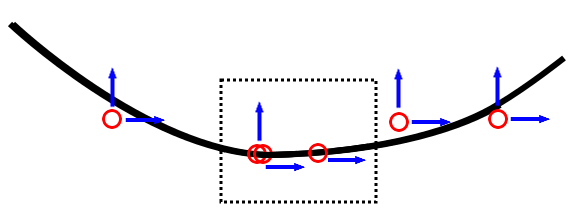
\includegraphics[scale=0.5]{figs/throat_area_control_points.png}
\end{center}
\end{figure}

\item[Wall thickness piecewise linear control points $w$] These control points are a set of coordinates between which a linear interpolation gives the shape of the thickness $t(\hat x)$ of the nozzle wall. The thickness of the wall is defined such that:

  \begin{equation}
  R_{wall,outer}(\hat x) = R_{wall,inner}(\hat x) + t(\hat x)
  \end{equation}

Each control point denotes the x-position and height (relative y-position) of the exterior nozzle wall from the interior nozzle wall. A linear interpolation is used between control points.
\end{description}

\subsubsection{Supporting structure}
The supporting structure consists of longerons and baffles which carry structural and thermal loads from the nozzle to the surrounding aircraft structure. The variables that can be adjusted will be written here shortly.

\subsubsection{Material}
The material properties of the nozzle greatly influence the heat transfer, stresses, and strength of the nozzle. A constant density material is assumed.
\begin{description}
\item[Thermal conductivity $k$] This parameter describes how resistant the material is to the transfer of heat.
\item[Thermal expansion coefficient $\alpha$] This parameter describes how much the material expands when subjected to a temperature difference and is related to the thermal stresses in the material.
\item[Elastic modulus $E$] This parameter describes the stiffness of the material.
\item[Yield stress $\sigma_{y}$] This parameter is the maximum allowable amount of stress the material can be subjected to without yielding. We choose it to be fixed for all temperatures.
\item[Max allowable temperature $T_{max}$] This parameter is the maximum allowable temperature the material can be subjected to.
\end{description}

\subsubsection{Inlet Conditions}
The boundary condition on the inlet of the nozzle is assumed to be uniform flow, although it can be stochastic. The stagnation pressure and temperature of the inlet flow is governed by the upstream engine turbine and other components and is dependent on the operating conditions.
\begin{description}
\item[Inlet stagnation temperature $T_{stag}$] 
\item[Inlet stagnation pressure $P_{stag}$]
\end{description}

\subsubsection{Environment}
The environment the engine is operating in is dependent on the mission. Freestream temperature and pressure will vary with altitude. The heat transfer coefficient will also vary with speed.
\begin{description}
\item[Heat transfer coefficient from external nozzle wall to ambient $h_{\infty}$] A lot of complicated physics is lumped into this one parameter, but it does have a large effect on the heat transfer through the nozzle wall.
\item[Freestream temperature $T_{\infty}$]
\item[Freestream pressure $P_{\infty}$]
\end{description}

\subsection{Ranges}

Table \ref{tab:variableRanges} summarizes reasonable ranges and nominal values of the aforementioned variables.

\begin{landscape}

\begin{table}
\caption{Ranges for nozzle design variables}
\label{tab:variableRanges}
\begin{center}
\begin{tabular}[]{p{4cm} | c | c | c | c}
Variable & Name in F100-nozzle Code & Minimum & Nominal & Maximum \\
\hline
\textbf{Geometry}\footnote{baseline geometry is provided in the \texttt{driveNozzle.m} script} & & & & \\ \hline
Interior wall B-spline control points $c$ & \texttt{nozzle.geometry.bSpline.coefs} & ~-20\% & baseline shape & ~+20\% \\ \hline
Wall thickness piecewise linear control points $w$ & \texttt{nozzle.wall.seed} & ~-20\% & baseline shape & ~+20\% \\ \hline
\hline
\textbf{Supporting Structure} & & & & \\ \hline
\hline
\textbf{Material}\footnote{material properties for SEPCARBINOX A500, a ceramic matrix composite} & & & & \\ \hline
Thermal conductivity $k$ (W/m-K) & \texttt{nozzle.wall.k} & -10\% & 8.6 & +10\% \\ \hline
Thermal expansion coefficient $\alpha$ (1/K) & \texttt{nozzle.wall.coeffThermalExpansion} & -10\% & 2.3e-6 & +10\% \\ \hline
Elastic modulus $E$ (Pa) & \texttt{nozzle.wall.E} & -10\% & 80e9 & +10\% \\ \hline
Yield stress $\sigma_y$ (Pa) & N/A & & & \\ \hline
Max allowable temperature $T_{max}$ (K) & N/A & & & \\ \hline
\hline
\textbf{Inlet Conditions} & & & & \\ \hline
Inlet stagnation temperature $T_{stag}$ (K) & \texttt{nozzle.inlet.Tstag} & -5\% & mission dependent & +5\% \\ \hline
Inlet stagnation pressure $P_{stag}$ (Pa) & \texttt{nozzle.inlet.Pstag} & -10\% & mission dependent & +10\% \\ \hline
\hline
\textbf{Environment} & & & & \\ \hline
Heat transfer coefficient from external nozzle wall to ambient $h_{\infty}$ (W/$\textrm{m}^2$-K) & \texttt{nozzle.hInf} & ~20? & 25? & 500 \\ \hline
Freestream temperature $T_{\infty}$ (K) & \texttt{freestream.T} & -5\% & mission dependent & +5\% \\ \hline
Freestream pressure $P_{\infty}$ (Pa) & \texttt{freestream.P} & -5\% & mission dependent & +5\% \\ \hline
\hline
\end{tabular}
\end{center}
\end{table}

\end{landscape}

\section{Quantities of Interest}

For the nozzle design problem, there are a handful of important quantities of interest. Depending on whether stochastic design variables or parameters are used, the quantities of interest may be deterministic or stochastic. Stochastic quantities of interest can also include the mean, variance, or cumulative distribution functions (CDF).

\begin{description}
\item[Weight $W$] This quantity is solely determined by the geometric variables, namely the control points of the interior wall's B-spline $c$ and the control points of the piecewise-linear thickness function $w$.
\item[Thrust $T$] This quantity is affected by a wide range of variables and is most sensitive inlet stagnation pressures, temperatures, as well as geometry changes near the throat and exit.
\item[\# Cycles to failure $N_f$] This quantity takes $T_w$ and $\sigma_1$ into account during its calculations and is affected by a wide range of variables.
\item[Max wall temperature $max( T_w )$] This quantity is primarily governed by the inlet stagnation temperature and heat transfer at the wall.
\item[Largest principal stress $max( \sigma_1 )$] This quantity is primarily governed by the thermal stresses in the wall.
\end{description}

\section{Problem Formulations}

The problem presented in equation \ref{eq:generalFormulation} is not the only possible nozzle design problem formulation, although it is the one we are currently pursuing. Here we review other formulations, as well as more details about the formulation of constraints in equation \ref{eq:generalFormulation}.

\subsection{Other Formulations}

\subsubsection{Maximum Lifetime}

A maximum lifetime optimization would emphasize the reliability of the nozzle over its lifetime.

\begin{equation}
\label{eq:maxLifetimeFormulation}
%\mathbbm{P}_1 \begin{cases}
\begin{aligned}
& \underset{x}{\text{maximize}}
% objective function:
& & N_f  \\
& \text{subject to}
% constraints:
& & W(x) < c_1 \\
& & & P [ T(x,\xi) \geq T_{req} ] > c_2 \\
& & & P [ max( T_w (x,\xi) ) \leq T_{max} ] > c_3 \\
& & & P [ max( \sigma_1 (x,\xi) ) \leq \sigma_{y} ] > c_4 \\
& & & A x \leq b \\
& & & l \leq x \leq u \\
\end{aligned}
%\end{cases}
\end{equation}

where $x = \irow{c^T & w^T}^T$ or in other words all of the geometric variables. The uncertain parameters could be $\xi = \irow{ k & \alpha & E & T_{stag} & P_{stag} & h_{\infty} & T_{\infty} & P_{\infty} }^T$.

\subsubsection{Minimum Overall Consumer Cost}

A minimum overall consumer cost optimization would attempt to minimize the total financial impact of the nozzle over its lifetime, including design, manufacturing, maintenance, and disposal.

\begin{equation}
\label{eq:minCostFormulation}
%\mathbbm{P}_1 \begin{cases}
\begin{aligned}
& \underset{x}{\text{maximize}}
% objective function:
& & \beta_1 f_1(W(x)) + E[ \beta_2 f_2(sfc(x,\xi)) + \beta_3 f_3(N_f(x,\xi)) ]  \\
& \text{subject to}
% constraints:
& & P [ T(x,\xi) \geq T_{req} ] > c_1 \\
& & & A x \leq b \\
& & & l \leq x \leq u \\
\end{aligned}
%\end{cases}
\end{equation}

where $\beta_i$ are weights for each function $f_i()$. The objective function is essentially a surrogate function for estimating the average total cost of the nozzle over its lifetime and beyond. Since nozzle failures will be manifested as high costs, negatively impacting the objective, the number of constraints is much lower. For this formulation, $x = \irow{c^T & w^T}^T$ again and the uncertain parameters could be $\xi = \irow{ k & \alpha & E & T_{stag} & P_{stag} & h_{\infty} & T_{\infty} & P_{\infty} }^T$. 

\subsubsection{Materials Selection}

As an extension to the above formulations, a materials selection and mixed programming optimization problem could be implemented instead by setting the design variables $x = \irow{ k & \alpha & E & \sigma_y & T_{max} }^T$ and using any combination of uncertain parameters $\xi$.

\subsection{Form of Stochastic Objective \& Constraints}

Stochastic objectives can be implemented in several forms:
\begin{description}
\item[Mean] For example, $E[W]$ where $E[\dots]$ denotes expectation.
\item[Mean with variance penalty] For example, $E[W] + \kappa \sigma(W)$ where $\kappa$ is a constant and $\sigma(\dots)$ denotes the standard deviation.
\item[Percentile requirement] For example, $P[W < W_{req}]$.
\item[CDF matching] For example, $RI(W) = \int_\Omega \vert F_W (W) - \delta_W (RAO) \vert d \xi$. See Petrone, Iaccarino, Quagliarella 2011 for more details.
\end{description}

While formulating a deterministic constraint is relatively straightforward, there are several forms a robust stochastic constraint could take:

\begin{description}
\item[Moment constraint] For example, $E[T] - 3 \sigma(T) > T_{req}$ where $E[\dots]$ denotes expectation and $\sigma(\dots)$ the standard deviation. This form inherently assumes an approximately normally-distributed quantity of interest.
\item[Chance constraint] For example, $P[T > T_{req}] > 0.99$.
\end{description}

\subsection{Linear Constraints}
\label{sec:linearConstraints}

Linear constraints on the geometric design variables are important for obtaining reasonable shapes. Linear constraints are only discussed here for the design variables corresponding to the coordinates of the interior wall's B-spline coefficients. Thus, taking the design variable vector $x = \irow{ c }$, where $c$ contains all non-duplicated coordinates from the B-spline coefficient matrix, a set of linear constraints $A x \leq b$ should be implemented in any optimization. The matrix $A$ includes the following constraints:

\begin{enumerate}
\item The x-coordinates of neighboring control points should not crossover each other. 
\item The pre-throat geometry should converge monotonically, not diverge.
\item The control points governing the nozzle throat should remain below all other control points.
\item The absolute value of the slope of the line drawn between two adjacent control points should be less than a certain value (this is a surrogate for limiting the slope of the B-spline itself). 
\end{enumerate}

In addition, in order to avoid numerical difficulties, all B-spline control points should be separated by a small $\delta$, say $\delta = 1e-2 \textrm{ or } 1e-3$.

\section{Results}

\subsection{Deterministic}

\subsubsection{Simplified Minimum Weight, Low-fidelity Model}

The following simplified deterministic minimum weight problem was solved using NPSOL as called from Dakota:

\begin{equation}
\label{eq:minWeightLowFiSimplified}
%\mathbbm{P}_1 \begin{cases}
\begin{aligned}
& \underset{x}{\text{minimize}}
% objective function:
& & W(x) \\
& \text{subject to}
% constraints:
& & T(x) \geq 25,000 \\
& & & A x \leq b \\
& & & l \leq x \leq u \\
\end{aligned}
%\end{cases}
\end{equation}

where $x = \irow{w}$. The optimization was performed for mission 3, \textit{i.e} a flight regime of 35,000 ft and Mach 0.9. The convergence tolerance was 1e-8 and a forward finite difference step size of 1e-3 was used. The optimization began from the baseline nozzle geometry where a few linear constraints were not satisfied by a small amount.

\begin{figure}
\caption{Comparison of initial design and optimal design using the low-fidelity quasi-1D F100-nozzle code. Note that in order to minimize weight, the nozzle has been converted to a tube with a flare at the end to maintain thrust. Compression and expansion waves are not taken into account.}
\label{fig:minWeightLofiSimpleResults}
\begin{center}
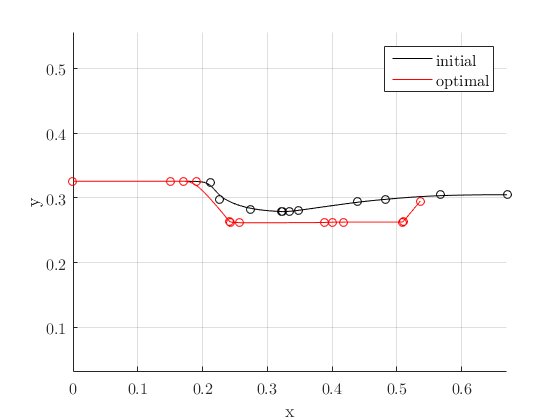
\includegraphics[scale=0.5]{figs/det_lowfi_result.png}
\end{center}
\end{figure}

The optimization converged in 68 minutes, 1012 function evaluations, and 25 major iterations with the termination message ``current point cannot be improved upon.'' Figure \ref{fig:minWeightLofiSimpleResults} compares the initial and final design. The optimal weight is 9,878 $\textrm{cm}^3$. The thrust constraint is tight, and 5 control points are pushed to their x-coordinate limits. Other tight linear constraints include the min/max slope constraints near the inlet and outlet of the nozzle, some throat remains the lowest point constraints, and a few relative x-position constraints.

\subsubsection{Simplified Minimum Weight, Med-fidelity Model}

The same optimization problem formulated in equation \ref{eq:minWeightLowFiSimplified} was solved using the medium-fidelity model using Euler CFD. The implementation was in Matlab using fmincon's SQP implementation. The convergence tolerance was 1e-6 and a forward finite difference step size of 1e-3 was used. The optimization began from a slightly modified baseline geometry with completely feasible constraints. Figure \ref{fig:minWeightMedfiSimpleResults} compares the initial and final design.

\begin{figure}
\caption{Comparison of initial design and optimal design using the med-fidelity Euler CFD calculations in SU2. Note that the shape of the nozzle is much more contoured than the low-fidelity result and a lower weight is achieved since there is favorable interaction between the geometry and the flow that results in higher thrust.}
\label{fig:minWeightMedfiSimpleResults}
\begin{center}
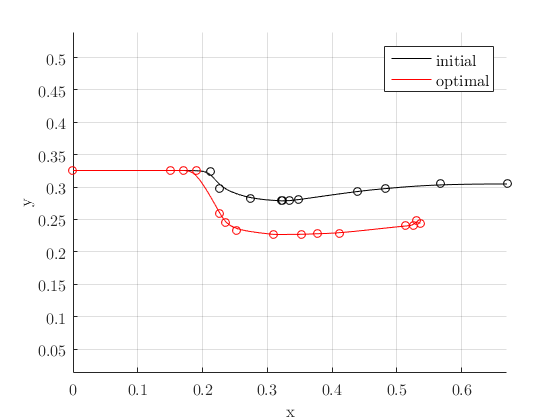
\includegraphics[scale=0.5]{figs/det_medfi_result.png}
\end{center}
\end{figure}

The optimization converged in 5.2 hours using fmincon's parallel mode and 12 processors with 31 total iterations. The optimization stopped since the relative maximum constraint violation was met (1e-6) and all changes in the design variables was less than the step tolerance (1e-6). The optimal weight is 9,199.08 $\textrm{cm}^3$. The optimal value of thrust was 25,012 N. 

\subsection{Stochastic}

\subsubsection{Control Variate Minimum Weight, Low-fidelity Model}

A simplified stochastic minimum weight optimization problem was formulated using a moment constraint on the thrust, as shown below. A control variate approach was used, where the high-fidelity evaluation was the low-fidelity quasi-1D nozzle code, and the low-fidelity evaluation was a Taylor series approximation of the low-fidelity nozzle code. 4 samples were used to calculate moments for the high-fidelity evaluation and 32 samples were used to calculate moments for the low-fidelity evaluation. 
 
\begin{equation}
\label{eq:minWeightCVLowFiSimplified}
%\mathbbm{P}_1 \begin{cases}
\begin{aligned}
& \underset{x}{\text{minimize}}
% objective function:
& & W(x) \\
& \text{subject to}
% constraints:
& & E[T(x,\xi)] - 3 \sigma(T(x,\xi)) \geq 25,000 \\
& & & A x \leq b \\
& & & l \leq x \leq u \\
\end{aligned}
%\end{cases}
\end{equation}

where $x = \irow{c}$ and $\xi = \irow{ T_{stag} & P_{stag} & T_{\infty} & P_{\infty} }^T$, where all the uncertain parameters were assumed to have normal distributions. NPSOL was used through Dakota with a convergence tolerance of 1e-8. Forward finite difference with a step size of 1e-3 was used. Figure \ref{fig:minWeightLofiCVSimpleResults} compares the initial and final design.

\begin{figure}
\caption{Comparison of initial design and optimal design using a control variate method on a stochastic minimum weight optimization problem. Note that the throat has been pushed up in order to provide adequate thrust over a larger range of conditions.}
\label{fig:minWeightLofiCVSimpleResults}
\begin{center}
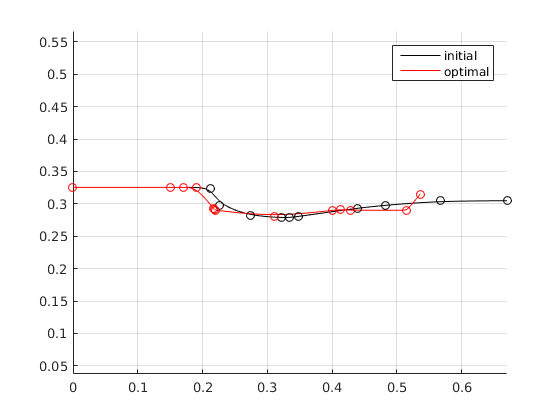
\includegraphics[scale=0.5]{figs/cv_lowfi_result.png}
\end{center}
\end{figure}

The optimization converged in about 30 minutes on 4 cores, 16 function evaluations, and 10 major iterations with the message ``current point cannot be improved upon.'' The optimal weight is 10,360.50 $\textrm{cm}^3$. The value of the thrust constraint at the optimum was 25,004.84 N. Other tight linear constraints included a cluster of 3 x-position constraints prior to the throat, 6 throat is lowest constraints, and 1 tight max slope constraint near the exit. In addition there are two extra constraints which are also active. These require the control points on either side of the throat to be close to the throat.

\subsubsection{Control Variate Minimum Weight, Med-fidelity Model}

Currently, there is difficulty in getting the optimization to converge while respecting the nonlinear thrust constraint.

\end{document}
